\documentclass{article}
\usepackage[dutch]{babel}
\usepackage{hyperref}
\usepackage{graphicx}
\usepackage[bottom=2.5cm, right=2.5cm, left=2.5cm, top=2.5cm]{geometry}

\title{Startvergadering ML sessie 6}
\author{Team $\exists$uler\\
	\textit{Daan, Marie, Zeineb, Florian, Vincent, Jasper, Lasha, Younes}}
\date{Vrijdag 17 november 2023}

\begin{document}
	
	\maketitle
	
	\section*{Stand van zaken}
	
	Afgelopen week werden alle simulaties en procedures van vorige sessie afgewerkt. In figuur \ref{fig:kanban} is de status van het tabblad \textit{Implementatie} te zien vóór de aanvang van deze 6e sessie.
	
	Bovendien programmeerde Vincent al een aantal zaken om voor de bijkomende toepassing \textit{Support Vector Machines}. Hij maakte eerst een SVM-model op een trainingsdataset met 30 onafhankelijke variabelen of x-waarden. Dit model kon zeer accuraat voorspellen of een tumor in de borst van een persoon al dan niet kwaadaardig was bij een validatie- en testdataset. Het probleem met het gebruiken van zo veel inputs, is echter dat we dit niet visueel kunnen voorstellen aangezien we in heel hoge dimensies werken. Daarom werd er ook een bestand aangemaakt waarin er slechts 2 inputs worden bekeken, zodat we de data mooi kunnen plotten. Dit alles kan teruggevonden worden in de subdirectory \textit{tumorclassificatie} in de map \textit{Implementatie}.
	
	\section*{Planning voor deze sessie}
	
	\subsection*{Bespreken van de simulaties en procedures}
	
	Deze sessie zullen we de simulaties en procedures van vorige sessie eerst en vooral met elkaar bespreken, zodat iedereen zeker op de hoogte is van wat er precies allemaal in de Python-files en Jupyter-notebooks staat. Het is belangrijk dat iedereen de geschreven code snapt. Op die manier kunnen we allemaal samen een coherent eindverslag maken en heeft iedereen genoeg kennis om tijdens de postersessie een woordje uitleg te kunnen geven.
	
	\subsection*{Uitwerken van de extra toepassing}
	
	Na het bespreken van de simulaties uit vorige sessie, zullen we ook eerst de toepassing rond de classificatie tumoren bespreken. Daarna zullen we voor deze toepassing simulaties uitvoeren, waarbij we telkens maar zullen kijken naar 2 inputs, aangezien we anders de data niet grafisch kunnen voorstellen. De zaken die in orde moeten worden gebracht, staan reeds in de KanBan en zijn te zien in figuur \ref{fig:kanban2}. Ieder teamlid kiest dus een taak uit deze lijst.
	
	\begin{figure}
		\centering
		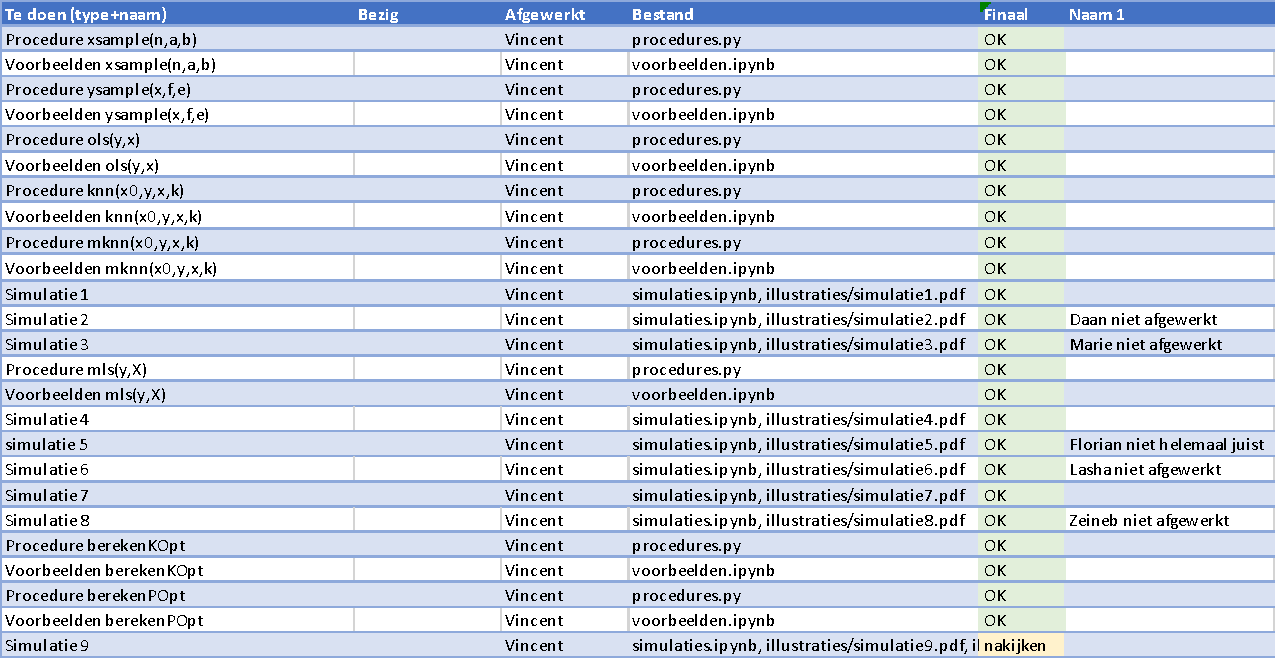
\includegraphics[width=1\textwidth]{kanban}
		\caption{De status van het tabblad \textit{Implementatie} in de KanBan vóór de aanvang van sessie 6.}
		\label{fig:kanban}
	\end{figure}
	
	\begin{figure}
		\centering
		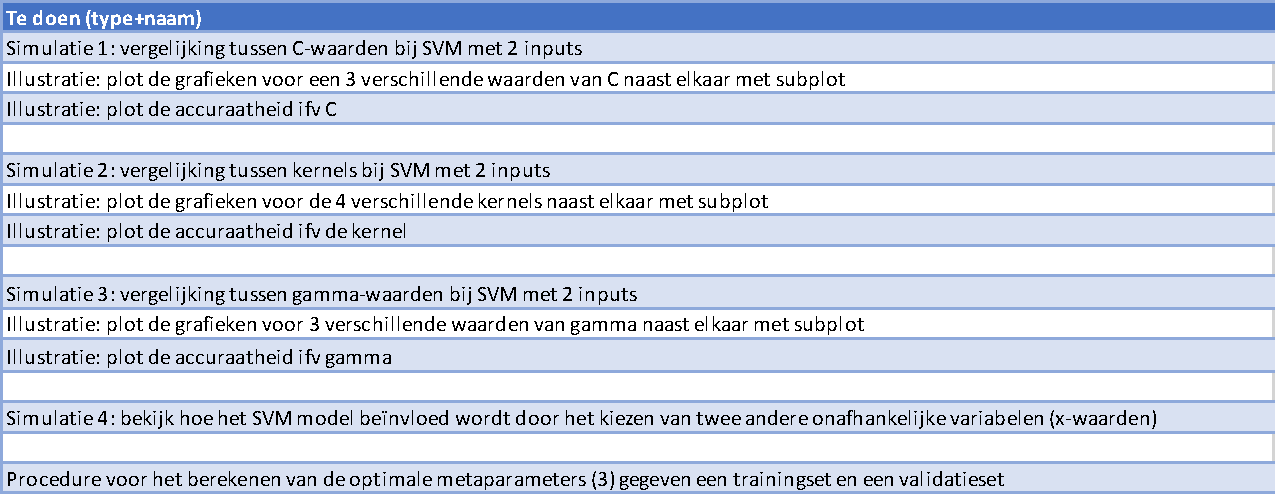
\includegraphics[width=1\textwidth]{kanban2}
		\caption{De planning voor sessie 6 in het tabblad \textit{Toepassing}.}
		\label{fig:kanban2}
	\end{figure}
	
\end{document}